	\documentclass{llncs}
	\usepackage{llncsdoc}
	\usepackage[noend]{algpseudocode}
	\usepackage{subfig} 
	\usepackage{graphicx}
	\usepackage{frame, caption}
	\usepackage{amsmath}
	\usepackage{eulervm}
	\usepackage{fontenc}
	\usepackage{mathrsfs}
	\usepackage{multirow, enumitem, longtable, rotating,lipsum, scrextend}
	\usepackage{array}
	\usepackage[rflt]{floatflt}
	\usepackage{makecell}	
	\usepackage{xcolor, soul}
	\sethlcolor{yellow}	
	\usepackage{floatrow}

	\setlength\extrarowheight{3pt}
	% Table float box with bottom caption, box width adjusted to content
	\newfloatcommand{capbtabbox}{table}[][\FBwidth]
	
	\begin{document}
	\title{\vskip -10pt Dominance in dialogue of collaborative negotiation}
	
	\author{Lydia Ould Ouali\inst{1}, Charles Rich\inst{2} \and
		Nicolas Sabouret\inst{1} }
	
	\institute{LIMSI-CNRS, UPR 3251, Orsay, France \\
		Universit\'e Paris-Sud, Orsay, France \\
		\email{\{ouldouali, nicolas.sabouret\}@limsi.fr}
		\and
		Worcester Polytechnic Institute\\ Worcester, Massachusetts, USA\\
		\email{rich@wpi.edu}
	}

	\maketitle
	
	\begin{abstract}
		This paper presents a model of conversational agent that can deploys different strategies of negotiation based on the social power it wants to express for the user. This model is based on three principles of collaborative negotiation from the literature in social psychology. We show that this principles are correctly perceived by a human observer: the social behavior of the agent is made visible through its dialogue strategy.
	\end{abstract}
	
	\section{Introduction}
	As artificial conversational agents become more and more popular, they became capable to hold a conversation with a human user and potentially collaborate with the user in order to achieve a common objective. For example, artificial tutors collaborate with students [\hl{ref}], or a companion agents can help elderly to follow a specific diet \cite{kidd2005sociable}. In this context, the user(s) and the agent have to negotiate in collaborative manner about the way to achieve the common task. This is called \emph{collaborative negotiation}. Unlike adversarial negotiation [\hl{ref-traum-marsella}], collaborative negotiation assumes that each participant is driven by the goal of finding a trade-off that best satisfies the interests of all the participants as a group, instead of one that maximizes his own interest\cite{sidnerartificial,chu1995response}.
	
	Moreover, previous research has shown that people tend to respond to computers as social actors \cite{bickmore2005establishing}. This led the IVA community to study the psychosocial relationship between the user and the agent during their interaction: a growing body of research is investigating the use of appropriate social behavior for virtual agents in different roles and types of user-computer relationship \cite{bickmore2005s,bickmore2005establishing,kidd2005sociable}. In the context of human-human communication involving negotiation, social psychology and communication \cite{dunbar2005perceptions,de1995impact} investigated the impact of social relations and emotion on the negotiation. They proved that  \emph{interpersonal power} directly affects the strategies of negotiators. Therefore, in order to build intelligent conversational agents that conduct good collaborative negotiations, it is very important to allow them to adapt their negotiation strategies to different levels of interpersonal power. [Traum et al. studied this question in the context of adversarial multi-party negotiation. We consider the case of collaborative one-to-one dialogue.]
	
	In this paper, we present a model of conversational agent that can deploys different strategies of negotiation based on the social power it wants to express for the user. In the next section, we discuss existing works on interpersonal power in the domain of social psychology and affective computing. Section 3 presents the negotiation model, based on a set of utterance types and a model of preferences. It implements three principles of collaborative negotiation from the literature in social psychology. In section 4, we present an experiment conducted with two virtual agents and we show that these principles are correctly perceived by a human observer.	
	
	\section{Related works}
	The notion of social power has been widely studied in the fields of interpersonal communication and psychology \cite{kecskes2013research}. It can be defined as the capacity to produce intended effects and ability to influence the behavior of other person in the conversation \cite{dunbar2005perceptions}. In the context of communication, power is a dyadic variable that takes place during the dialogue, where the interlocutor who exerts power is viewed as \textit{dominant}, while the interlocutor with low power's behaviors is viewed as \textit{submissive}. 
% where one individual's attempt of control is necessarily acquainted by the partner in the interaction.\cite{dunbar2005perceptions}

	Behaviors related to power can contribute either positively or negatively to the dialogue. Positive contributions include keeping the conversation going, making quick decisions, etc. Negative contributions include not considering the partner (\emph{e.g.} not giving the occasion to express his opinion), appearing offensive, etc. \cite{zablotskaya2012relating}. In our work, we focus on negotiation dialogues, for which several researchers already proved the impact of power on the negotiation \cite{van2006power}.
	
	\subsection*{Behaviors of power in dialogue}
	\label{domDialogue}
	During a conversation, power can manifest through verbal and nonverbal behaviors.	
	At the nonverbal level, a wide range of behaviors have been associated with the relation of power in kinestesic behaviors (facial expression, body movements and gestures) and voice (speaking duration, speaking intensity, voice control and pitch) \cite{burgoonnonverbal}. Based on this work, several IVA have been developped with the ability to exhibit social power through nonverbal behavior, such as gaze \cite{lance2008relation}, body movements \cite{mignault2003many} or head tilt \cite{gebhard2014exploring,callejas2014computational} in relation to power and submission perception. Similarly, \cite{strassmann2016effect} investigated the perception of nonverbal behaviors of virtual agents with a focus on power and cooperation.
	
	Verbal behaviors of power in the dialogue are related to the type of \textit{strategies} that individuals choose in order to take control of the other especially during a negotiation. A considerable body of research has documented the effects of power on negotiation behaviors and outcomes. De Dreu demonstrated that \cite{de1995impact} dominant negotiators have higher aspirations, demands more and concede less. Galinsky \cite{galinsky2003power} affirms that power increases the action orientation: dominant negotiators control the flow of the negotiation. In addition, high power increase task orientation and goal-directed behavior. \cite{giebels2000interdependence} shows that this leads dominant negotiators to end up with the larger share of the pie.
	
	Furthermore, power affects the way that negotiators gather information about their partners \cite{de2004influence}. Submissive negotiators have a stronger desire to develop an accurate understanding of their negotiation partner, which would lead them to ask more \emph{diagnostic} rather than \emph{leading} questions.
	
	It was also shown that dominant negotiators are self-centered and tend to not pay attention to the preferences of submissive negotiators \cite{fiske1993controlling,de1995impact}.
	%					 The idea is that high-dominant individuals have many resources and can often act at will without serious consequences, while submissive individuals, have to be more careful because they are more dependent on other people. In addition, they are motivated to gain or regain control over their outcomes by paying close attention to the people on whom they depend.
	%					

	In our work, we use a text-oriented dialogue system and we therefore focus on the verbal behaviors.  Our goal is to make visible \emph{the strategies} deployed during the negotiation depending on the power. In order to implement these different behaviors, we extracted three principle related to the relation of power that impact strategies of negotiation:
	\begin{enumerate}
	\item \textbf{Self Vs Other:} Submissive negotiators consider the preferences of other in the negotiation, whereas dominant negotiators  are self-centered and only interested by satisfying their own preferences. \cite{fiske1993controlling,de1995impact}
	
	\item \textbf{Representation of demands:} Dominant negotiators show a higher level of demand than the submissive ones. In addition,  Submissive negotiator's demand decrease over time, and tends to make larger concessions than dominant negotiators. \cite{de1995impact}
	
	\item \textbf{Control the flow of the negotiation:}
	Dominant negotiators tend to make the first move \cite{magee2007power}. In addition, they take the lead of the negotiation. Otherwise, submissive negotiators aim to construct an accurate model of other preferences, which lead them to ask more questions about other preferences rather than keeping the negotiation going (makes proposals). \cite{de2004influence}
	
	\end{enumerate}
	%	We will present in the next section the decision model based on the behaviors of power. 
	%						\item Based on Carsten, De Dreu and Van Kleef demonstrate that high power negotiators are high in their propensity to negotiate relative to participants with low power. (leading individuals to focus on the rewards available to them in situations and to bargain forgreater rewards than were initially offered to them.)			
	
	Only few models consider the expression of power in the verbal behavior of an IVA. \cite{bee2010bossy} developped an agent that expresses social dominance through gaze and linguistic features. They demonstrated that the linguistic personality traits influence the perception of power. However, this work does not consider the how power affects the strategies of negotiation in dialogue. More recently, [\hl{ref-traum}] consider trust and interaction management as dimensions of the negotiation strategy of a virtual agents. However, this research focuses more on the negotiation aspect than on the expression of social behaviour. Moreover, it considers only adversarial negotiation.
	
	
	\section{Model of negotiation based on the relation of power}
	In this section, we present our model of dialogue of negotiation of preferences.	
	First, we present the data structure for the agent's preferences and the topics of the negotiation. Second, we present the implementation of the principles of behaviors of power in negotiation (see section \ref{domDialogue}).

	\subsection{Domain model}
	The overall goal of a negotiation is to choose an \textbf{option} in a set of possible options $\mathcal{O}$. The evaluation of each option by participants is based on a set of \textbf{criteria} that reflect options characteristics. Let us consider a set $\mathcal{C}$ of $n$ criteria and let $C_1,\ldots,C_n$ be their respective domains of values. $\mathcal{O}$ can be simply defined as the cross-product $C_1\times\ldots\times C_n$ and each option $o\in\mathcal{O}$ is a tuple $(v_1,\ldots,v_n)\in\mathcal{O}$. For instance, in a dialogue about restaurants for which the criteria would be the type of cuisine and the price, we could have the option ``Chez Francis'' that is an expensive French restaurant: $francis=(French,expensive)$.
	
	\subsection{Preference model} 
	Each agent is provided with a set of preferences, defined as a set $\prec$ of partial orders $\prec_i$ on each $C_i$. For instance, if the agent prefers French food to Italian, $French\prec_{cuisine}Italian$.
	
	For a given value $v\in C_i$, the agent can compute the \emph{satisfaction} it has for this value as the number of ancestors in the preference order $\prec_i$, normalised in [0,1]:
	
	\begin{equation}
	sat_{self}(v, \prec_i) =	1 - \left( \frac{|\{d : d \neq c \  \wedge \ (v \prec_i d)\}| }{( |C_i| - 1 )}\right)
	\end{equation}
	
	This notion of satisfaction is generalized to any option $o=(v_1,\ldots,v_n) \in \mathcal{O}$ as a simple weighted sum\footnote{There exists a great amount of literature in theoretic decision making on how to combine multiple criteria using Order Weight Averages or Choquet's integrals, for instance. We are not concerned by this question of criteria agregation in this paper.}:
	\begin{equation}
	sat(o, \prec) = \frac{\sum_{i}^{n} sat(v_i, \prec_i) }{n}
	\end{equation}
	
	\subsection{Dialogue model}
	Negotiators communicate during the negotiation via utterance types (or speech acts). Each utterance type has a specific set of arguments and is associated with a natural language generation. We defined five main types of utterance, based on the work by Sidner \cite{sidnerartificial}, and three derivate types that are combinations of the main ones.
		
		\begin{table}[h]
			\begin{tabular} {|p{2.5cm}|p{3.5cm}|p{6cm}|}
				\hline
				Utterance type & parameters & NL generation\\
				\hline
				StatePreference & $v \in C_i$, $b\in\{True,False\}$ & I (don't) like /$v$/.\\
				\hline
				 \multirow{2}{*}{AskPreference} &$v \in C_i$ & Do you like /$v$/ ?\\
				 \cline{2-3} & $i\in\mathcal{C}$ & What kind of /$i$/ do you like ?\\
				 \hline
				 \multirow{2}{*}{Propose} & $o \in \mathcal{O}$ & Let's go to /$o$/.\\
				 \cline{2-3} & $v \in C_i$ & Let's go to a /$v$/ restaurant.\\
				 \hline
				 Accept& $x \in \mathcal{O} \vee x\in C_i$ & Okay, let's go to /$x$/.\\
				 \hline
				 Reject & $x \in \mathcal{O} \vee x\in C_i$ & I'd rather choose  something else. \\
				 \hline
				 \hline
				 RejectPropose & $(r,p)\in C_i^2 \vee (r,p) \in \mathcal{O}^2 $ & I don't want to go to $r$. Let's rather go to $p$ \\
				 \hline 
				 RejectState & $x \in \mathcal{O} \vee x\in C_i$ &  I don't like /$x$/, let's choose something else. \\
				 \hline
				 AcceptPropose & $o \in \mathcal{O}$ & Okay. Let's go to /$o$/.\\
				 \hline
			\end{tabular}
			\caption{The list of possible utterances in the model of dialogue}
		\end{table}
	
	The agent can ask information about the preferences of its interlocutor (Ask) or give information about its own preferences (State). It can propose, accept and reject both values of criteria (``Let's go to a Chinese restaurant'') or options (``Let's go to \emph{Chez Francis}''). The RejectPropose utterance type is used to clearly reject an option and make a counter-proposal in the same dialogue move. Similarly, the RejectState utterance type is used to make a reject with an explanation. The AcceptPropose is used to accept a criteria and propose a compatible option. Examples of dialogues are given in \hl{section} \ref{sec:expe}.
	
	\medskip
	The utterance selection algorithm is described in section \ref{sec:decision}. For the utterance selection, the agent keeps track of statements and proposals all along the dialogue. For each criteria $i\in\mathcal{C}$, we build the set $S_i \subseteq C_i$ of statements that the agent has made about this criteria. This avoids re-statements of previous information. We also have the sets $A_i$ and $U_i$ of values that have been stated by the interlocutor as satisfiable or not (using a \emph{State} utterance type). We assume that $A_i\cap U_i=\emptyset$ and $A_i\cup U_i\subseteq C_i$ (some values can still be unknown). These sets serve as a model of the interlocutor's preferences that evolves during the negotiation. From these, we can compute the satisfiability of a value $v\in C_i$ for the other as:
	
	\begin{equation}
	sat_{other}(v, A_i, U_i)= \left\{\begin{array}{ll}
	1	 & \mathrm{if\ }  c \in A_i\\
	0    & \mathrm{if\ }c \in U_i\\
	0.5	 & \mathrm{otherwise}
	\end{array}\right.
	\end{equation}
	
	This function is generalized to any option $o=(v_1,\ldots,v_n) \in O$ as a weighted sum:
	
	\begin{equation}
	sat_{other}(o, A, U) = \frac{ \sum_{i}^{n} other(v_i, A_i, U_i) } {n}
	\end{equation}
	
	We also maintain the sets $P_i \subseteq C_i$, $T_i\subseteq C_i$ and $R_i\subseteq C_i$ of all proposed, accepted and rejected values for each criteria. This will be used to make relevant proposals. Similarly, we consider $P\subseteq \mathcal{O}$, $T\subseteq \mathcal{O}$ and $R\subseteq \mathcal{O}$ the sets of all proposed, accepted and rejected options in the dialogue.
	

	\subsection{Decision based on power in negotiation}
	\label{sec:decision}
	We extracted from work in social psychology three mains principles related to the relation of power which affects negotiators strategies and behaviors (see section \ref{domDialogue}). We present in this section, the formal theory built for each principle. 
	
	\subsubsection{Level of demand and concessions}
	In collaborative negotiation, both participants reduce their level of demand in time because they want to reach an agreement. According to our second principle, the concessions should be higher for submissive agents. To implement this mechanism, we use a \emph{concession curve}, as illustrated on figure \ref{fig:concession}.
	
	 \begin{figure}[t]
		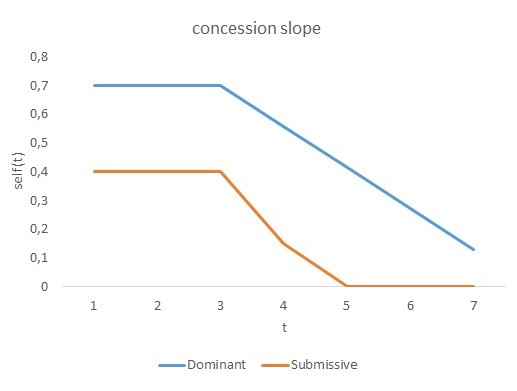
\includegraphics[width=.4\linewidth,keepaspectratio=true]{graphs/slope.jpg}
		\caption{\label{fig:concession}Concession curve for a dominant and a submissive agent}
	 \end{figure}
	 
	 This mechanism is defined as follows. Let $pow \in [0, 1] $ be the agent's initial power. It is a constant for a given agent in a given relationship. Let $self(pow, t)$ be the instant value of power, following the concession curve:
	 
	 \begin{equation}
	 self(pow, t) = \left\{\begin{array}{ll}
	 pow & \mathrm{if\ } (t \leq \tau)\\
	 max(0, pow - (\frac{\delta}{pow} . (t - \tau))) & \mathrm{otherwise}
	 \end{array}\right.
	 \end{equation}
	 
	 where is $t \geq 0$ is the number of open or rejected proposals and $\tau > 0$ and $\delta > 0$
	 are parameters of the theory (in our experiments, we use $\tau=2$ and $\delta=0.1$). This value $self$ represents the weight an agent gives to its self satisfaction in time.
	 
	 The acceptability of a value $v \in C_i$ is defined as a boolean function:
	 \begin{equation}
	 acc(v, t) = sat_{self}(v, \prec_i) \geq  \beta . Self(t).
	 \end{equation}
	 
	 with $\beta>0$ a parameter of the theory (we used $\beta=1$ in our implementation).
	 
	 This function is generalized to any option $o \in O$:
	 \begin{equation}
	 acc(o, t) = sat_{self}(o, \prec) \geq  \beta . Self(t)
	 \end{equation}
	
	\subsubsection {Self vs other}
	According to our first principle, dominant negotiators give more weight to the satisfaction of their own preferences. To implement this principle in the context of collaborative negotiation, we compute how much a given proposal is \emph{tolerable} considering the satisfiability for both the agent and its interlocutor.
	
	For a given criteria $i\in\mathcal{C}$, let $V_i\subseteq C_i$ be the subset of values that are acceptable for the agent:

	\begin{equation}
	V_i(t) = \{ v\in C_i : acc(v,t) \}
	\end{equation}
	
	We compute the tolerability of a given value $v\in V_i$ at a time $t$ knowing the preference order $\prec_i$ and the preference of the interlocutor:
	
	\begin{equation}
	\begin{split}
	tolerable(v, t, \prec_i, A_i, U_i, pow) & = self(pow, t) . sat_{self}(v, \prec_i) \\
	& +  (1 - self(pow, t)) . sat_{other}(v, A_i, U_i)
	\end{split} 
	\end{equation}
	
	And we generalize this function to any option $o=(v_1,\ldots,v_n) \in O$:
	
	\begin{equation}
	tolerable(o, t, \prec, A, U, pow) = \frac{ \sum_{i}^{n} tolerable(v_i, t, \prec_i, A_i, U_i, pow) } {n}
	\end{equation}
	
	
	\subsubsection{Lead of the negotiation}
	According to our third principle, dominant negotiators tend to lead the negotiation. We implemented this principle through the choice of utterance types described on table \ref{utt}. A dominant agent will focus on keeping the negotiation going by choosing \emph{negotiation moves} (Propose, Reject, Accept, RejectPropose or AcceptPropose). On the contrary, a submissive negotiator will focus on building an accurate model of other preferences in order to take the fairest decision. It will focus more on \emph{statement moves} (StatePreference, AskPeference or RejectState).
	
	We define a threshold $\pi$ to split the spectrum of power in two (dominant or submissive). We describe on table \ref{utt} the rules for utterance selection. Depending on the power, the previous utterance type (represented by $u^{-1}$) and the current dialogue state, the agent will select the first utterance type for which the condition is satisfied. For instance, a dominant agent will stop the negotiation as soon as all the remaining options are unacceptable (second line). A submissive agent will reject and state a preference, so as to explain why the proposal is not acceptable (third line of the submissive agent). If there is no open proposal, the submissive agent will propose any know acceptable criteria (4th line) or ask for new information (5th line).
	
	\begin{table}[t]
	\centering
	\begin{tabular}{|p{.45cm}|p{3cm}|p{8cm}|}
	\hline
	\parbox[t]{2mm}{\multirow{5}{*}{\rotatebox[origin=c]{90}{\textbf{pow  $>\pi$}}}}&\textbf{Utterance type} & \textbf{Condition} \\
	\cline{2-3}
	&Negotiation success & $\exists o \in T\cup P$, $acc(o,t) = true$ \\
	\cline{2-3}
	& Negotiation failure & $ \forall o \in \mathcal{O}, acc(o,t) = false$\\
	\cline{2-3}
	& State & $type(u^{-1}) = AskPreference \land n < \alpha$ \newline where $n$ is the number of successive statement moves and $\alpha$ a simulation parameter\\
	\cline{2-3}
	& AcceptPropose & $\exists i\in\mathcal{C}, \exists c \in P_i$, $acc(c,t)= true$ \\
	\cline{2-3}
	& RejectPropose & $\exists i\in\mathcal{C}, \exists c \in P_i$, $acc(c,t)= false$ \\
	\cline{2-3}
	& Propose & Otherwise  \\
	
	\hline
	\end{tabular}

	\begin{tabular}{|p{.45cm}|p{3cm}|p{8cm}|}
	\hline
	\parbox[t]{2mm}{
	\multirow{5}{*}{\rotatebox[origin=c]{90}{ \textbf{pow  $ \leq \pi$}}}} & \textbf{Utterance type} & \textbf{Condition} \\
	\cline{2-3}
	& Negotiation success &  $\exists o \in T$ \\
	\cline{2-3}
	& Accept & $\exists i\in\mathcal{C}, \exists c \in P_i, acc(c, t)=true   \lor \exists o \in P, acc(o, t) = true$ \\
	\cline{2-3}
	& RejectState & $ t<\tau \land (\exists i\in\mathcal{C}, \exists c \in P_i, acc(c, t) = false  \lor \exists o \in P,  acc(o, t)=false) $.\\
	\cline{2-3}
	& Propose & \hspace{1mm} $\exists i\in\mathcal{C}, \exists c \in C_i, sat_{other}(c, A_i, U_i)  = 1  \land acc(c, t)=true $
	\newline  $\lor \hspace{1.5mm}\forall i\in\mathcal{C},\exists c \in C_i, c \in T_i $\\
	\cline{2-3}
	& Ask & \hspace{3mm} $t > \tau \land \exists i\in\mathcal{C}, \exists c \in P_i, acc(c, t)=false$
	\newline $\lor \hspace{1.5mm}\exists i\in\mathcal{C}, \forall c \in C_i, sat_{other}(c, A_i, U_i)=0.5$\\
	
	\cline{2-3}
	
	& State & $\exists i\in\mathcal{C}, C_i\cap S_i \neq \emptyset$
	\\
	\cline{2-3}
	& Propose & Otherwise \\
	\hline
	\end{tabular}
	\caption{Selection of utterance types}
	\label{utt}
	\end{table}
	
	\section{Evaluation}
	
	In order to validate our model, we conducted a perceptual study in which participants have to determine the behaviors of two agents generated using our model. We have implemented the model in the DISCO \cite{rich} architecture and we generated synthetic dialogues betwen two artificial agents with different values of power and preferences.

\subsection{Study design}

	\hl{[NICO: remettre ici les valeurs de $\tau$, $\pi$, $\alpha$, $\beta$ et $\delta$.]}

	We implemented two conversational agents (\textit{speaker a} and \textit{speaker b}) which have to negotiate about a social topic of "negotiation about a restaurant where to have dinner".
	We generated a set of dialogues where we manipulated two conditions. First, the initial value of the power \textbf{pow} (see section \ref{decision}). 
	Speaker a will adopt a dominant negotiator's behaviors, while \textit{speaker b} will behave as a submissive negotiator. Therefore, power of \textit{speaker a} is initiated $pow>\pi$, complementarity \textit{speaker b} is initiated $ pow\leq \pi$.
	
	
	The second condition involved varying the initial preferences of both agents. We used the metric of Kendall distance \cite{bra2013Kendall} in order to compute the distance between two preferences sets. We manipulated the initial preferences to be either \textit{similar} or \textit{different}.
	The conditions manipulated to generate the dialogues are depicted in table \ref{Conditions}. An example of dialogue is presented in figure \ref{fig}
	
	\fbox{\begin{minipage}{0.9\textwidth}
			\begin{addmargin}[1em]{2em}% 1em left, 2em right
				A: "Let's go to a restaurant on the north side."
				
				B: "Okay, let's go to a restaurant on the north side."
				
				A: "Let's go to the Paris bistro . It's a romantic, cheap French restaurant on the north side."
				
				B: "Okay, let's go to the Paris bistro restaurant."
			\end{addmargin}

		\end{minipage}}
		
	
		
	\begin{table}
		\centering
		\begin{tabular}{ |l|c|c|l| }
			\hline
			\multicolumn{3}{ |c| }{Conditions} & \multirow{2}{*}{Dialogue's label}  \\ \cline{1-3}
			
			\newline \multirow{2}{*} {\textbf{Initial preferences}}& \multicolumn{2}{ c| } {\textbf{Dominance}} & \\ \cline{2-3}
			
			\newline  & pow(\textit{speaker a}) & pow(\textit{speaker b}) &  \\ 
			\hline
			\newline\multirow{3}{*} {Different preferences} & 0.9 & 0.4 & Dialogue 1 \\ \cline{2-4}
			
			\newline  & 0.7 & 0.4 & Dialogue 2\\ \cline{2-4}
			
			\newline   &0.7 & 0.2 & Dialogue 3\\ 
			\hline
			\newline Similar preferences & 0.7 & 0.4 & Dialogue 4\\
			\hline
		\end{tabular}
		\caption{Initial condition's setting for generating dialogues} 
		\label{Conditions}
	\end{table}
	
	\subsection{Hypotheses}
	We investigated four main hypotheses about the perception of agents behaviors of power during the negotiation. 
	\begin{itemize}
		\item  \textbf{H1:} The dominant speaker will more strongly be perceived as self-centered.  
		
		\item \textbf{H2:} The submissive speaker will be more strongly perceived as making larger concessions.
		
		\item \textbf{H3:}  The dominant speaker will more strongly be perceived as having a higher level of demand comparing to the submissive speaker.
		
		\item \textbf{H4:}  The dominant speaker will more strongly be perceived as taking the lead of the negotiation.
		
	\end{itemize}
	
	\subsection{Experimental Procedure}
	
	We conducted a between-subject study using an online crowdsoursing website \emph{CrowdFlower} \footnote{https://www.crowdflower.com/}. 
	Each participant was shown only one dialogue (see an example dialogue in ), where the task was to judge each agent behaviors. Agents were described as two friends trying to find a restaurant where to have dinner. %We wanted to avoid skewing the participant's perception by the fact that negotiators are artificial agents. 
	Participants were invited to read the assigned dialogue and answer the corresponding questionnaire. 
	
	We defined for each hypothesis two questions to analyze the speaker's behaviors related to the hypothesis. 
	Two test questions were included to check the sanity of the answers. Therefore, the questionnaire was defined with 18 questions. (see table \ref{questionnaire})
	
	\begin{table}
		\begin{tabular}{|p{1.5cm}|p{5cm}|p{7cm}|}
			\hline
			Hypothesis &question 1& question 2 \\
			\hline
			\textbf{H1} &Speaker (A/B) is self-centered. &Speaker (A/B) takes his friend's preferences into account in the choice of the restaurant.\\
			\hline
			\textbf{H2} &Speaker (A/B) makes concessions in the negotiation.&Speaker (A/B) gives up his position in the negotiation\\
			\hline
			\textbf{H3} & Speaker (A/B) is demanding&Speaker (A/B) presses his position in the negotiation. \\
			\hline
			\textbf{H4} &Speaker (A/B) takes the lead in the negotiation.&Speaker (A/B) takes the initiative in the negotiation \\
			\hline
		\end{tabular}
		\caption{List of questions asked for the questionnaire}
		\label{questionnaire}
	\end{table}
	A total of 120 subjects participated to the experiment. Each subject received \textit{25 cents}. 
	We limited the participant pools to native English speakers. We excluded participants providing wrong answers to our sanity questions. The final number of accepted participants was 105. 
	%Each generated dialogue had a questionnaire. There were 12 questions (including 2 test questions).
	\subsection{Results and discussion}
	Table  \ref{res} summarize the results of our study, which strongly support all of our four hypotheses.  In order to analyze our data, we first computed the correlation for each pair of questions (see table ). The obtained results showed a high correlation between each pair of questions for all the hypotheses. This allow us to compute the comparison between speakers behaviors in the different dialogues. We used a non parametric test of Wilcoxon signed-rank test for paired data.  
	Hypothesis \textbf{H1} stated that participants would perceive dominant speaker to be self-centered and only care about its own preferences. Our analysis confirmed our prediction. In all the dialogues, participants perceived \textit{speaker a} to be self-centered, whereas \textit{speaker b} was perceived as taking into account the preferences of the other speaker.
	
	Hypothesis \textbf{H2} predicted that the submissive speaker will be perceived to make larger concessions. For all the proposed dialogues, participants responses supported our hypothesis.
	Participants rated the level of demand of the dominant speaker (\textit{\textit{speaker a}})  to be significantly higher than \textit{speaker b}. This difference supports the hypothesis \textbf{H3}. 
	In addition, the analysis revealed a significant main effect of the power in the lead of the dialogue, indicating that participants perceived \textit{speaker a}  as more leading the dialogue \textit{speaker b} supporting highly hypothesis \textbf{H4}.  
	
	Finally, we made a post-study analysis to study the behaviors of power in the spectrum of power. We supposed that the highest the power gets in the spectrum, the better behaviors of power will be perceived. We did compare participant's judgments of \textit{speaker a} in dialogues where \textit{speaker a} had different setting of power whereas \textit{speaker b} had the same setting, which are \emph{Dialogue 1} and \emph{Dialogue 2}.
	The obtained results did not supported our hypothesis. no significant difference in agents behaviors was observed. This might be explained by the interpersonal nature of power, which means that participants rated the power of \textit{speaker a} in opposition of  \textit{speaker b's} behavior, which makes the comparison of agents behaviors from different dialogues irrelevant. 
	
	\begin{table}[t]
		
		\begin{tabular}{|ll|c|c|c|c|c|c|c|c|} 
			\cline{3-10}
			
			\multicolumn{1}{c} {}	& \multirow{2}{*} {}& \multicolumn{2}{c|} {Dialogue1} & \multicolumn{2}{c|} {Dialogue2} & \multicolumn{2}{c|} {Dialogue3} &\multicolumn{2}{c|} {Dialogue4} \\ 
			\cline{3-10}
			
			
			\multicolumn{1}{c} {} & & Agent1 & Agent2 & Agent1 & Agent2 & Agent1 & Agent2 & Agent1 & Agent2 \\
			\hline 
			%\multicolumn{9}{|c|}{ \textbf{Results for H1}} \\
			%	\hline
			\newline \multirow{2}{*} {\textbf{H1}}  & \multicolumn{1}{|l|}{ \textit{Mean} $\pm$ \textit{SD} } & 3.9 $\pm$ 1.1 & 2.2$\pm$ 0.9  & 3.6 $\pm$0.9 & 2.2 $\pm$0.8  &2.8 $\pm$1.1  & 2.13$\pm$ 0.7 & 3.4 $\pm$ 1 & 2 $\pm$0.9 \\
			\cline{2-10}	
			\newline & \multicolumn{1}{|l|}{p-value} & \multicolumn{2}{c|}{ $<<0.01$} & \multicolumn{2}{c|}{ $<<0.01$} & \multicolumn{2}{c|}{ $<0.01$}& \multicolumn{2}{c|}{ $<<0.01$}\\
			\hline	
			
			\newline \multirow{2}{*} {\textbf{H2}} &\multicolumn{1}{|l|}{ \textit{Mean} $\pm$ \textit{SD} } & 2.2 $\pm$ 1.1 & 4.3$\pm$ 0.8  & 2.5 $\pm$1.2 & 3.8 $\pm$1.04 &2.7 $\pm$1.2  & 3.6$\pm$ 0.8 & 2.3 $\pm$ 1 & 3.2 $\pm$1.2 \\
			\cline{2-10}	
			\newline & \multicolumn{1}{|l|}{p-value} & \multicolumn{2}{c|}{ $<<0.01$} & \multicolumn{2}{c|}{ $<<0.01$} & \multicolumn{2}{c|}{ $=0.01$}& \multicolumn{2}{c|}{ $<<0.01$}\\
			\hline	
			
			\newline \multirow{2}{*} {\textbf{H3}} &\multicolumn{1}{|l|}{ \textit{Mean} $\pm$ \textit{SD} } & 4.1 $\pm$ 0.8 & 2.6$\pm$ 1.1 & 4.03 $\pm$ 0.8 & 2.7 $\pm$0.9 &3.5 $\pm$1.1 & 2.3$\pm$ 1 & 3.8 $\pm$ 1.8 & 1.8 $\pm$0.8 \\
			\cline{2-10}	
			\newline & \multicolumn{1}{|l|}{p-value}  & \multicolumn{2}{c|}{ $<<0.01$} & \multicolumn{2}{c|}{ $<<0.01$} & \multicolumn{2}{c|}{ $<0.01$}& \multicolumn{2}{c|}{ $<<0.01$}\\
			\hline	
			%				
			
			
			\newline \multirow{2}{*} {\textbf{H4}} & \multicolumn{1}{|l|}{ \textit{Mean} $\pm$ \textit{SD} } & 4.2 $\pm$ 0.9 & 2.3$\pm$ 1.1  & 3.8 $\pm$0.9 & 2.6 $\pm$1.07 & 3.8 $\pm$0.9  & 2.8$\pm$ 1.1  & 4.5 $\pm$0.5  & 1.9 $\pm$ 0.9\\
			\cline{2-10}
			\newline & \multicolumn{1}{|l|}{p-value} & \multicolumn{2}{c|}{ $<<0.01$} & \multicolumn{2}{c|}{ $<<0.01$} & \multicolumn{2}{c|}{ $<0.05$}& \multicolumn{2}{c|}{ $<<0.01$}\\
			\hline	
		\end{tabular}
		\caption{Summary of the obtained results for each hypothesis}
		\label{res}
	\end{table}
	
	\subsection{Conclusion}
%	Our research aims to model a conversational agent which is able to deploy strategies of negotiation in function of its representation of power. 
%	We proposed a model which allows a conversational agent to generate strategies of negotiation in function of its interpersonal relation of power.
%	We extracted from research in social psychology three principles of negotiation behaviors related to power that we implemented.  
%	
%	Our on-line study had the purpose to validate the implemented behaviors and did provide strong support to the claim that the relation of power affects agent's behaviors in negotiation.
%	
%	We found that participants perceived a significant difference in the agent's behaviors depending on their respective relation of power.  
%	Indeed, all of our four hypotheses were confirmed. 
%	%We predicted that agents with higher power will be perceived as more individualist and self-centered, whereas agents with lower power would care about other preferences. Furthermore, agents with lower power were perceived to make larger concessions than did agents with higher power. Consistent with this prediction, agents with higher power showed a greater level of demand in the negotiation. Finally, we obtain evidence that agents with higher power tends to lead the dialogue and take control of the negotiation's flow. 
%	
%	Our findings validate our model of dialogue in general and specifically confirmed the coherence of the generated behaviors of power. 
%	The next step, would be to experiment our model in a realistic human-agent interaction.
%	Further on, the interaction with a user should take into consideration the user's representation of its relation with the agent. Therefore, we aim to extend our model with a module of theory of mind that would allow the agent to have a mental representation of the user, and by consequence adapt its behavior to complement the user behavior perceived during the dialogue.
%		

	
	% ================== BIBLIO ===============
	\vskip 4pt
	\bibliographystyle{plain}
	\small{\bibliography{Library}}



	\end{document}